\documentclass{beamer}

\usepackage[utf8]{inputenc}

\usetheme{Madrid}
\usecolortheme{beaver}

\usepackage{graphicx} % for importing images in figures - you definitely want this!
\usepackage{physics}
\usepackage{amsmath}
\usepackage{graphicx}       % Use pdf, png, jpg, or eps§ with pdflatex; use eps in DVI mode
\usepackage{wrapfig}
\usepackage{tabularx}
\usepackage{array}
\usepackage{tabu}
\usepackage{subfig}
\usepackage{etoolbox}% http://ctan.org/pkg/etoolbox
\AtBeginEnvironment{figure}{\setcounter{subfigure}{0}}% Resets subfigure counter at start of figure environment
\usepackage{bm}
\usepackage{tikz}

\newcommand{\backupbegin}{
   \newcounter{finalframe}
   \setcounter{finalframe}{\value{framenumber}}
}
\newcommand{\backupend}{
   \setcounter{framenumber}{\value{finalframe}}
}

\graphicspath{{images/}}

\title[SRG Exploration in 1-D]{Exploring Many-Body Force Induction in the Similarity Renormalization Group in 1 Dimension}
\author{Matthias Heinz}
\institute{The Ohio State University}
\date{Apr 11, 2018}

\setbeamertemplate{navigation symbols}{}
\begin{document}

%%%%%%%%%%%%%%%%%%%%%%%
% TITLE SLIDE
%%%%%%%%%%%%%%%%%%%%%%%
{%
% \setbeamertemplate{headline}{}
\begin{frame}
    \titlepage
    % \textcolor{OSUscarlet}{See arXiv:1704.03308}\\
    \begin{center}
        % \scriptsize{Building on Furnstahl, Klco, Phillips, Wesolowski, J.\ Phys.\ G \textbf{42}, 034028 (2015)}
        \scriptsize{Thesis Committee: Prof. Richard Furnstahl, Prof. Robert Perry, Prof. P Sadayappan}
    \end{center}
\end{frame}

\begin{frame}
\frametitle{Goals of Low-Energy Nuclear Theory}
\begin{itemize}
    \item Model atomic nuclei and calculate observables like ground state and excited state energies, nuclear radii, half-lives for different decays
    \item Model nuclear matter to better understand the structure of astrophysical systems like neutron stars
    \item Use accurate models of nuclear systems to aid in the search for beyond Standard Model physics
    \item Leverage improved understanding of nuclear physics in a variety of applications
\end{itemize}
\end{frame}


\begin{frame}
\frametitle{Challenge: The Interaction}
The first challenge of low-energy nuclear theory is due to the nature of inter-nucleon forces, which are given by the strong interaction:
\begin{itemize}
    \item Underlying theory, quantum chromodynamics, cannot be solved in closed form at low energies
    \item Modern 2-body and 3-body potentials are determined from scattering experiments and few-body nuclei
    \item Hard repulsive core couples low and high-energy parts of Hamiltonian
    % \item Show figure of AV18 s channel
\end{itemize}
\begin{center}
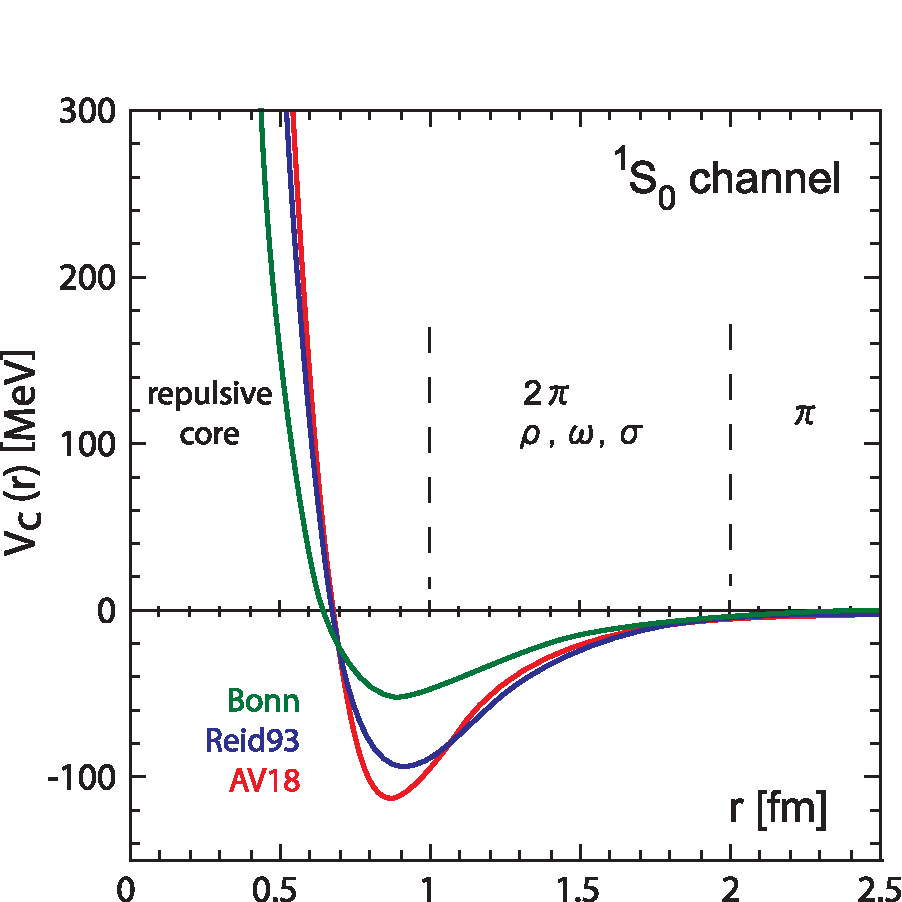
\includegraphics[width=0.36\textwidth]{hatsuda_phen-pot_new}

\tiny From R.J. Furnstahl, Nucl. Phys. Proc. Suppl. 228 (2012)
\end{center}
\end{frame}

\begin{frame}
\frametitle{Challenge: The Problem Size}
The second challenge of low-energy nuclear theory is that naive approaches quickly become intractable because of the rapid growth of the problem size:
\begin{itemize}
    \item Basis size grows combinatorially with respect to $A$, the number of particles
    \item Sets limit on what nuclei can be modeled, even when taking advantage of the most modern parallel computing clusters
    \item Strong off-diagonal couplings prevent significant basis truncation
\end{itemize}
\begin{center}
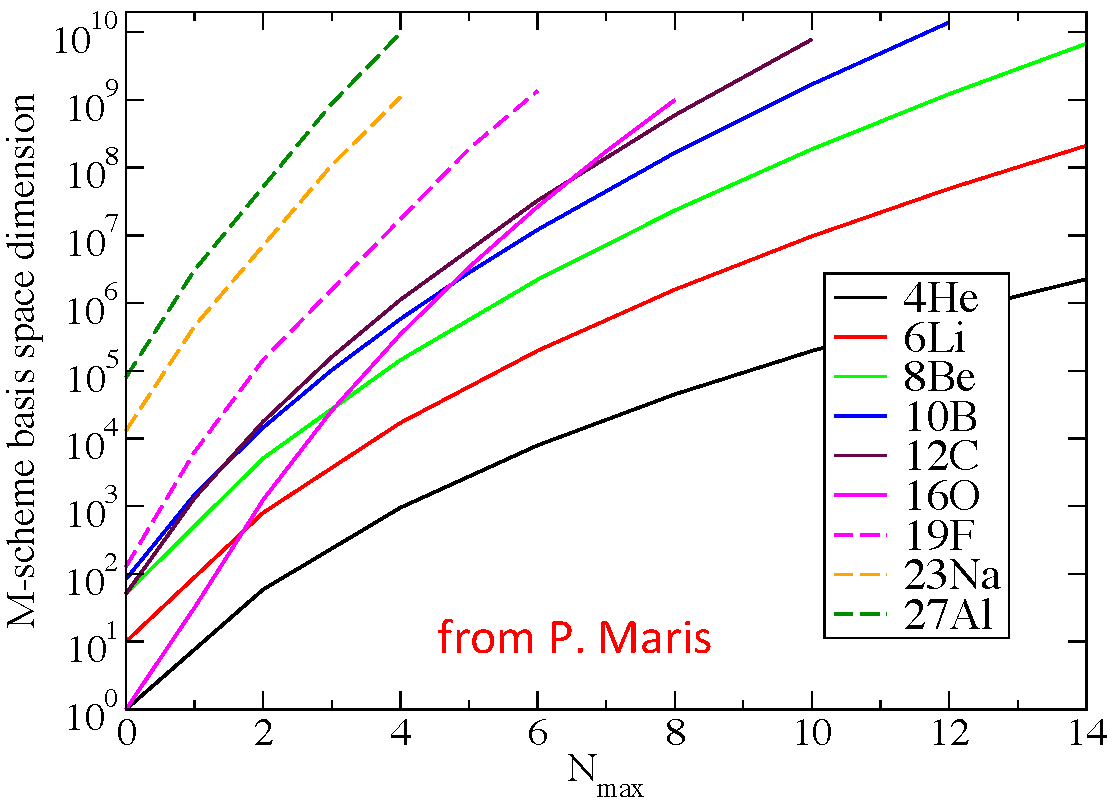
\includegraphics[width=0.38\textwidth]{maris_m-scheme_dimension_ack}

\tiny From P. Maris
\end{center}
\end{frame}

\begin{frame}
\frametitle{Recent Ab-Initio Explosion}
Range of nuclei able to be modeled via ab-initio methods (starting from inter-nucleon forces) has rapidly expanded due to effective field theory (EFT) and renormalization group (RG) methods:

\begin{center}
\begin{tikzpicture}
\node<1> (img1) {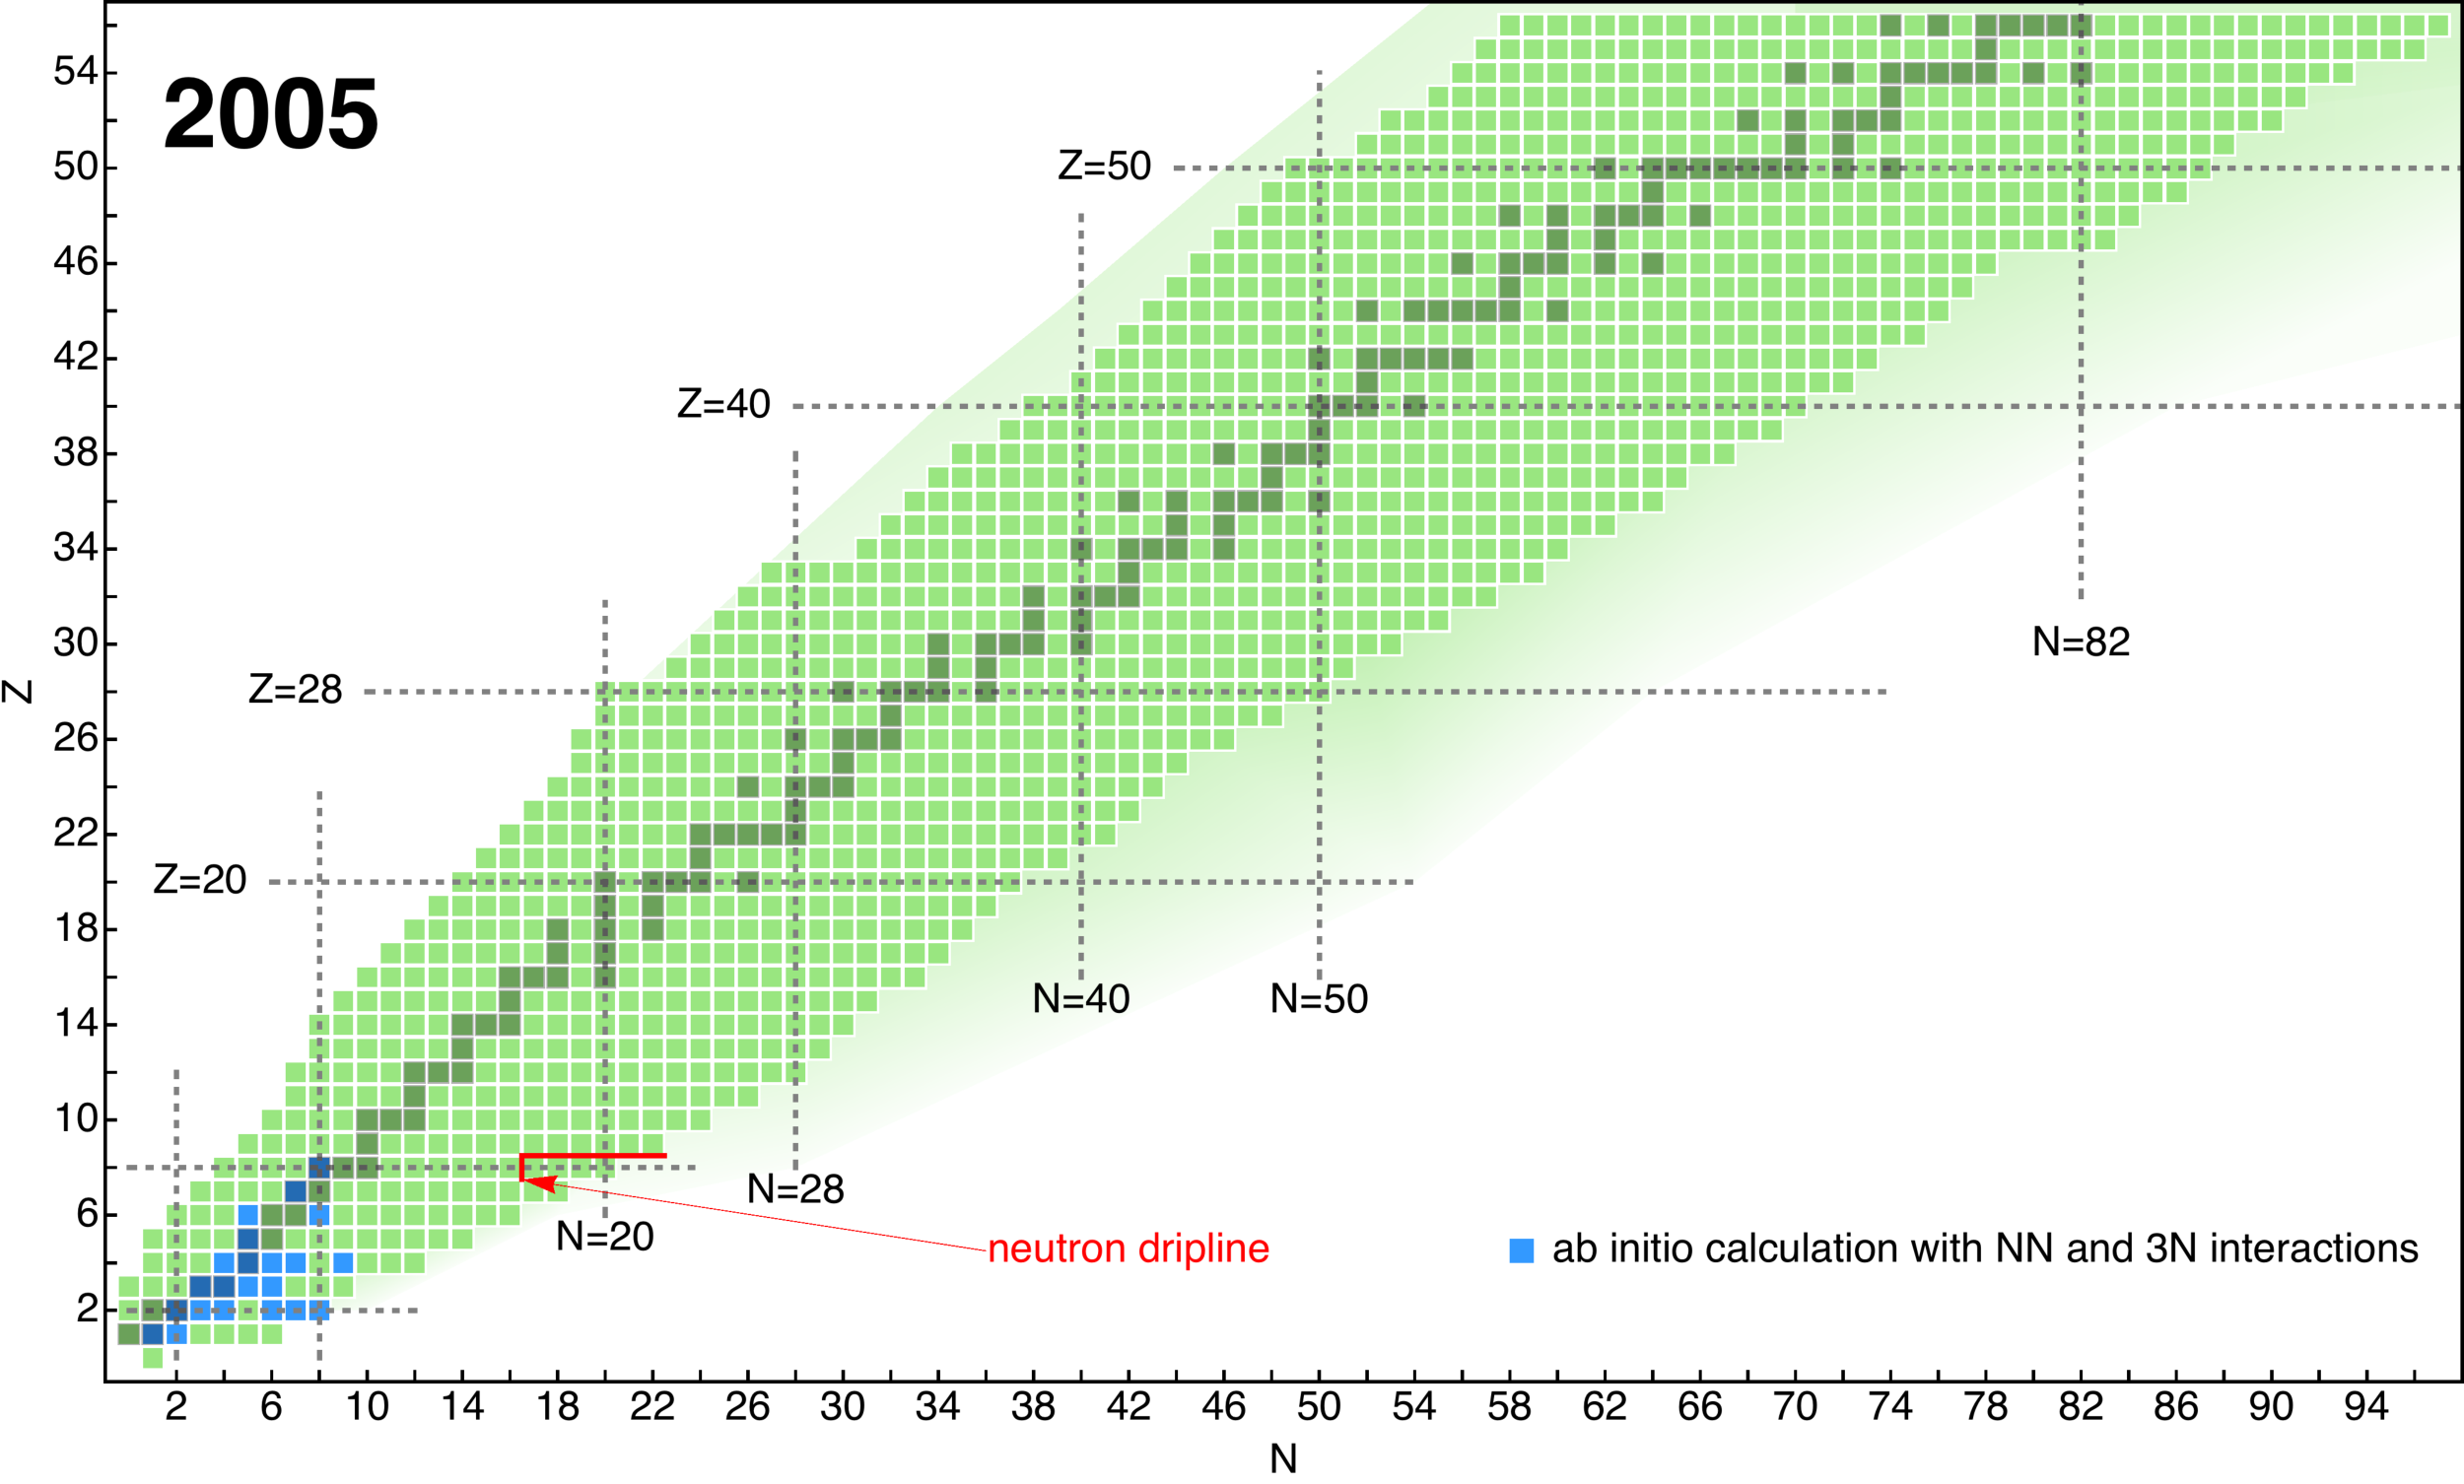
\includegraphics[width=0.8\textwidth]{nuclear_chart_2005}};
\node<2> (img2) {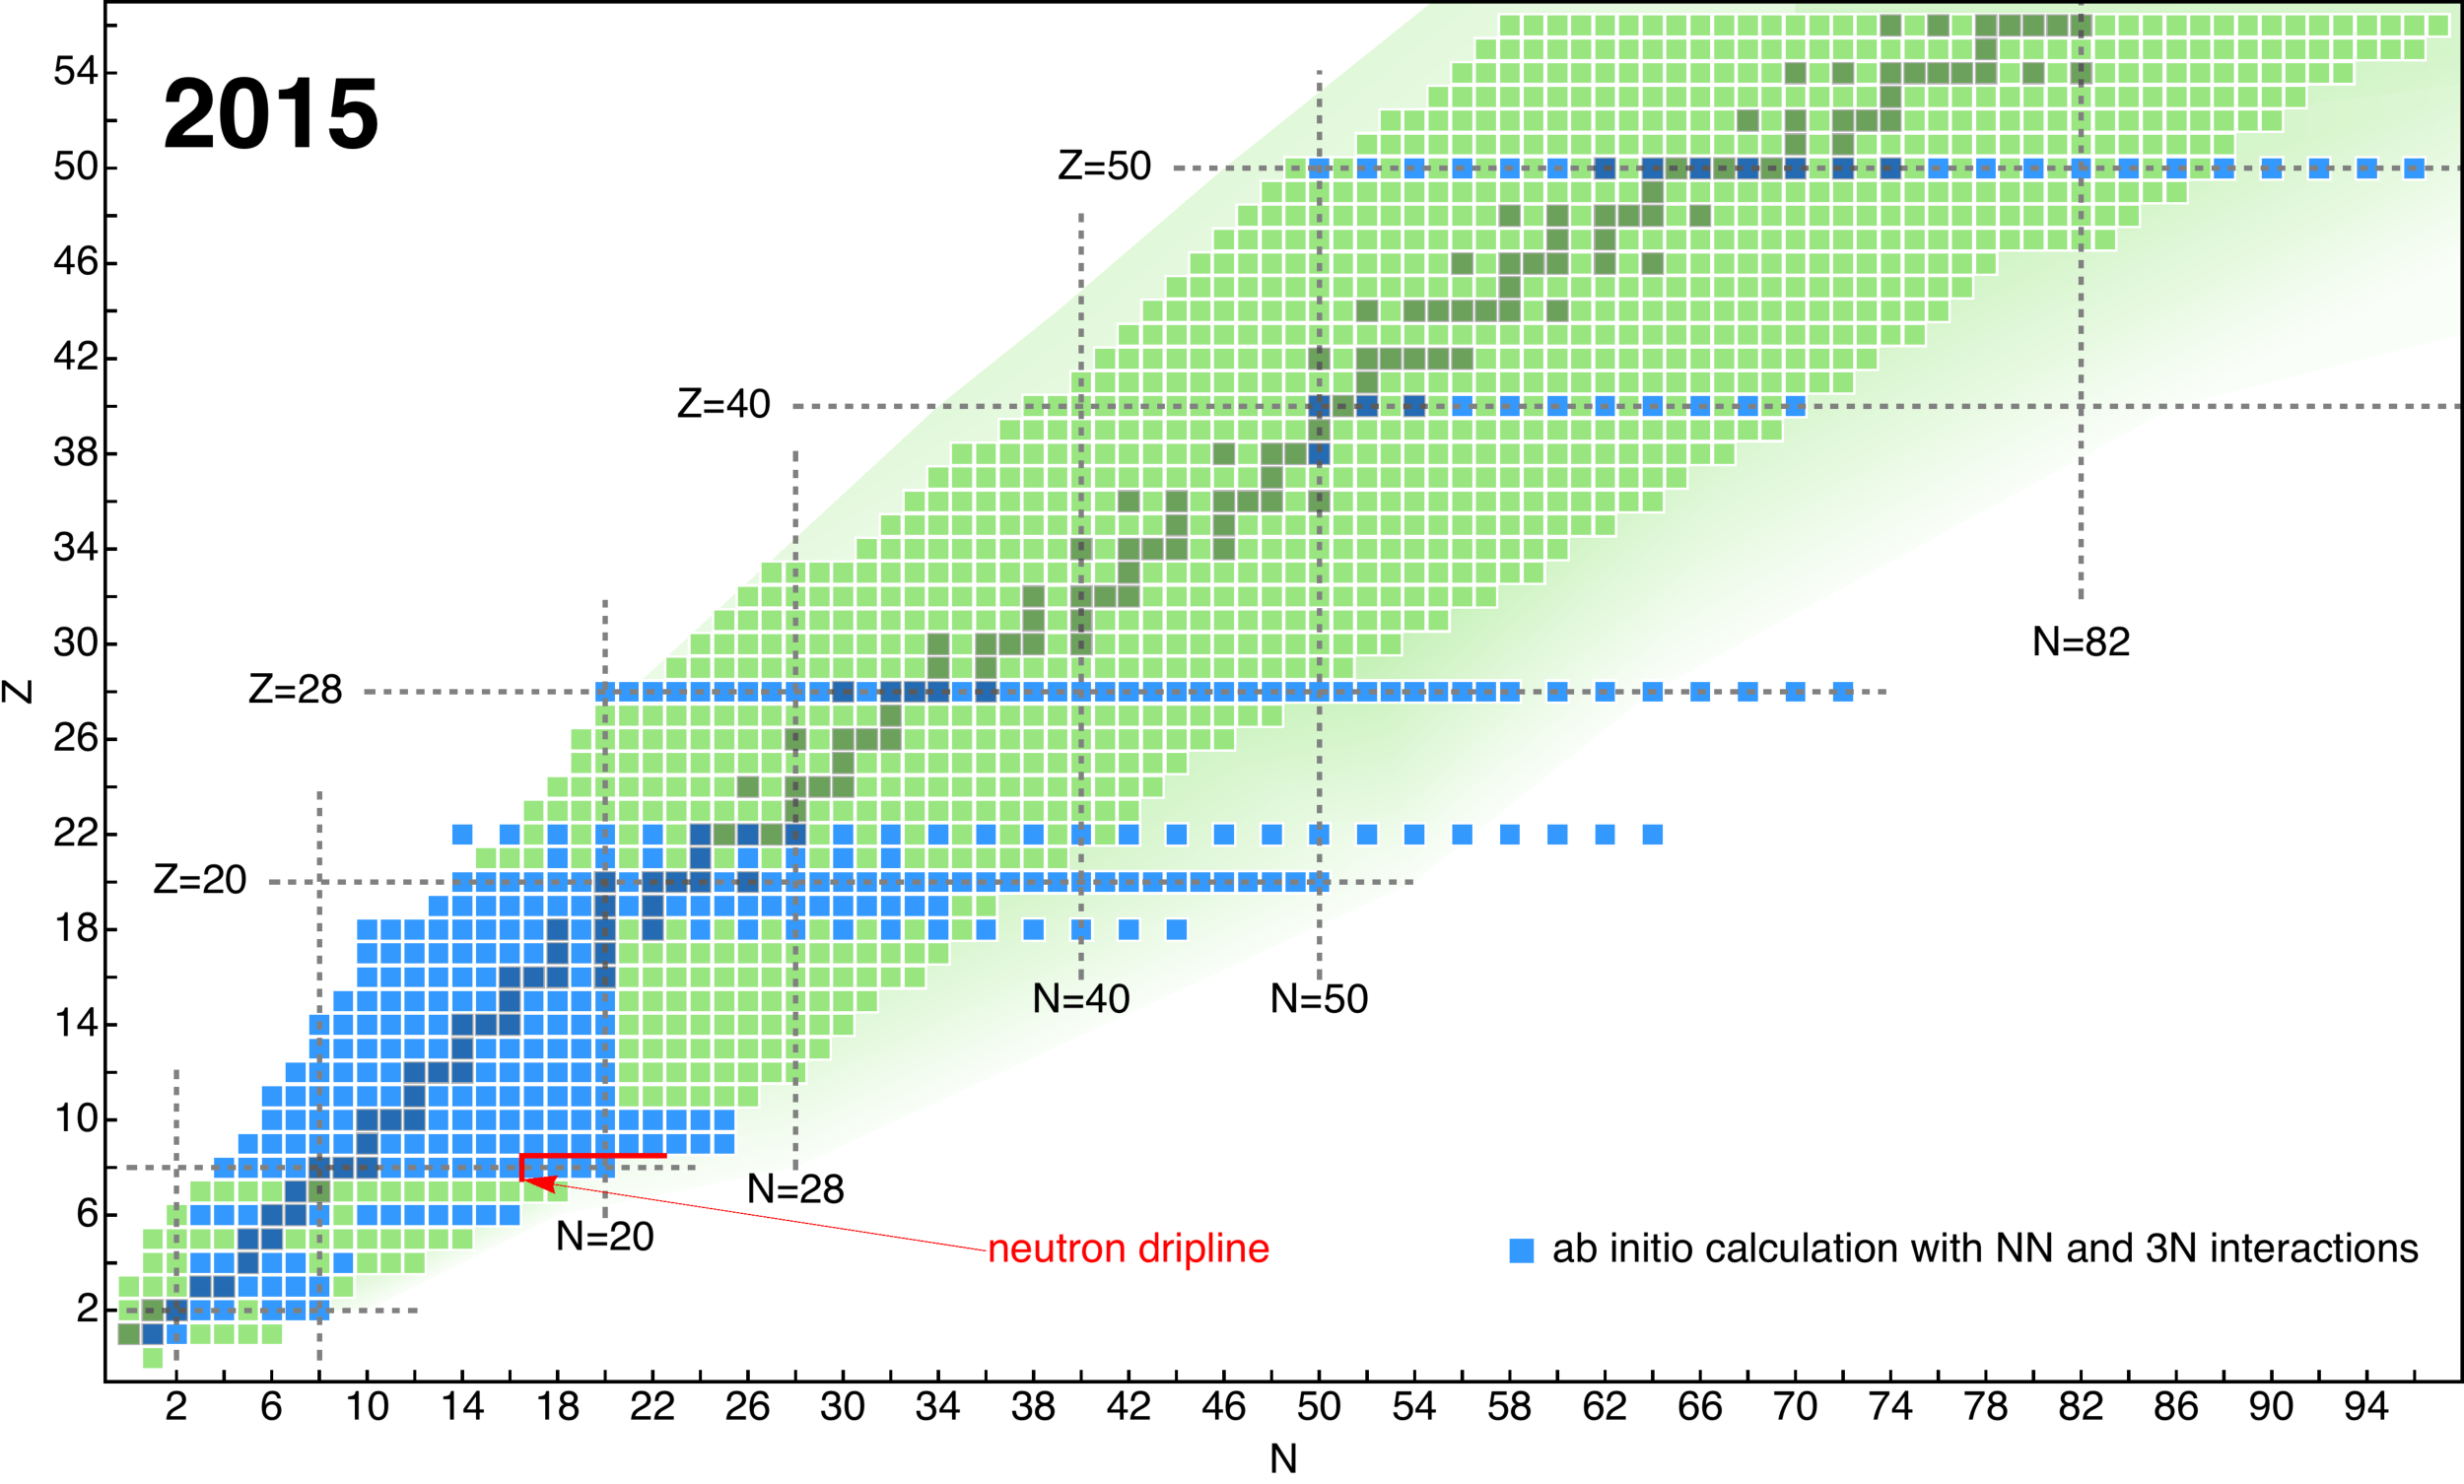
\includegraphics[width=0.8\textwidth]{nuclear_chart_2015}};
\node<3> (img3) {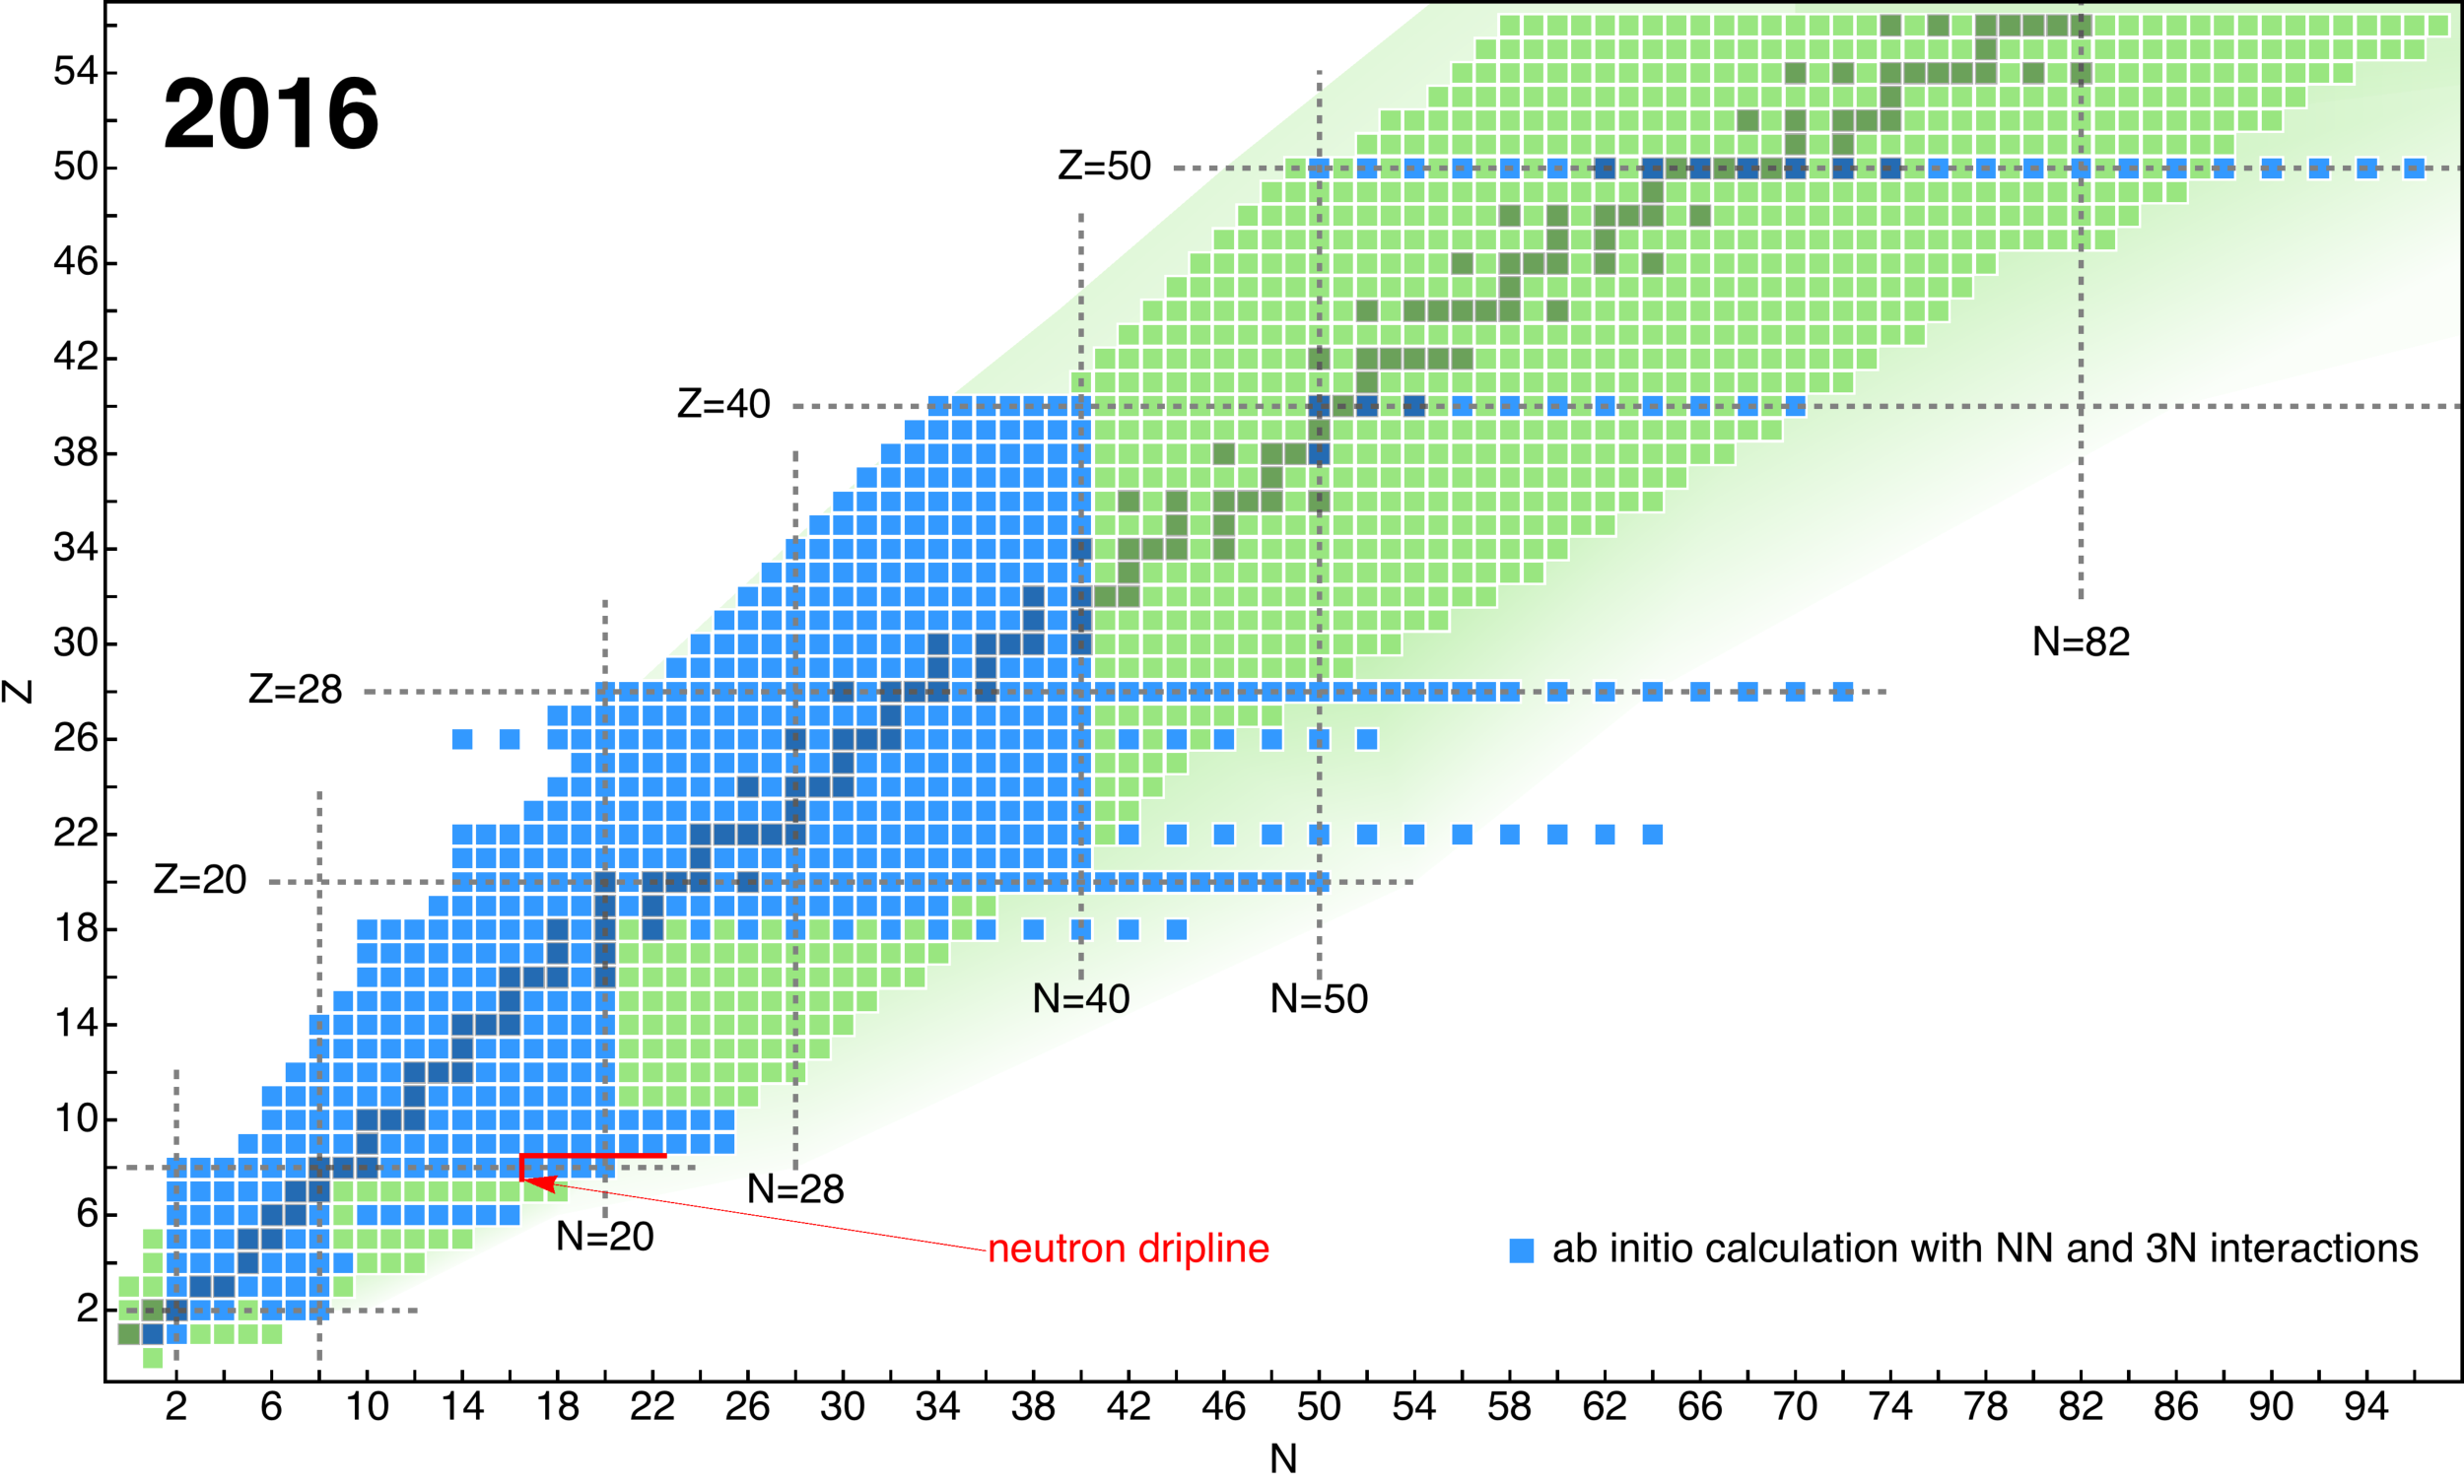
\includegraphics[width=0.8\textwidth]{nuclear_chart_2016}};
\node<4> (img4) {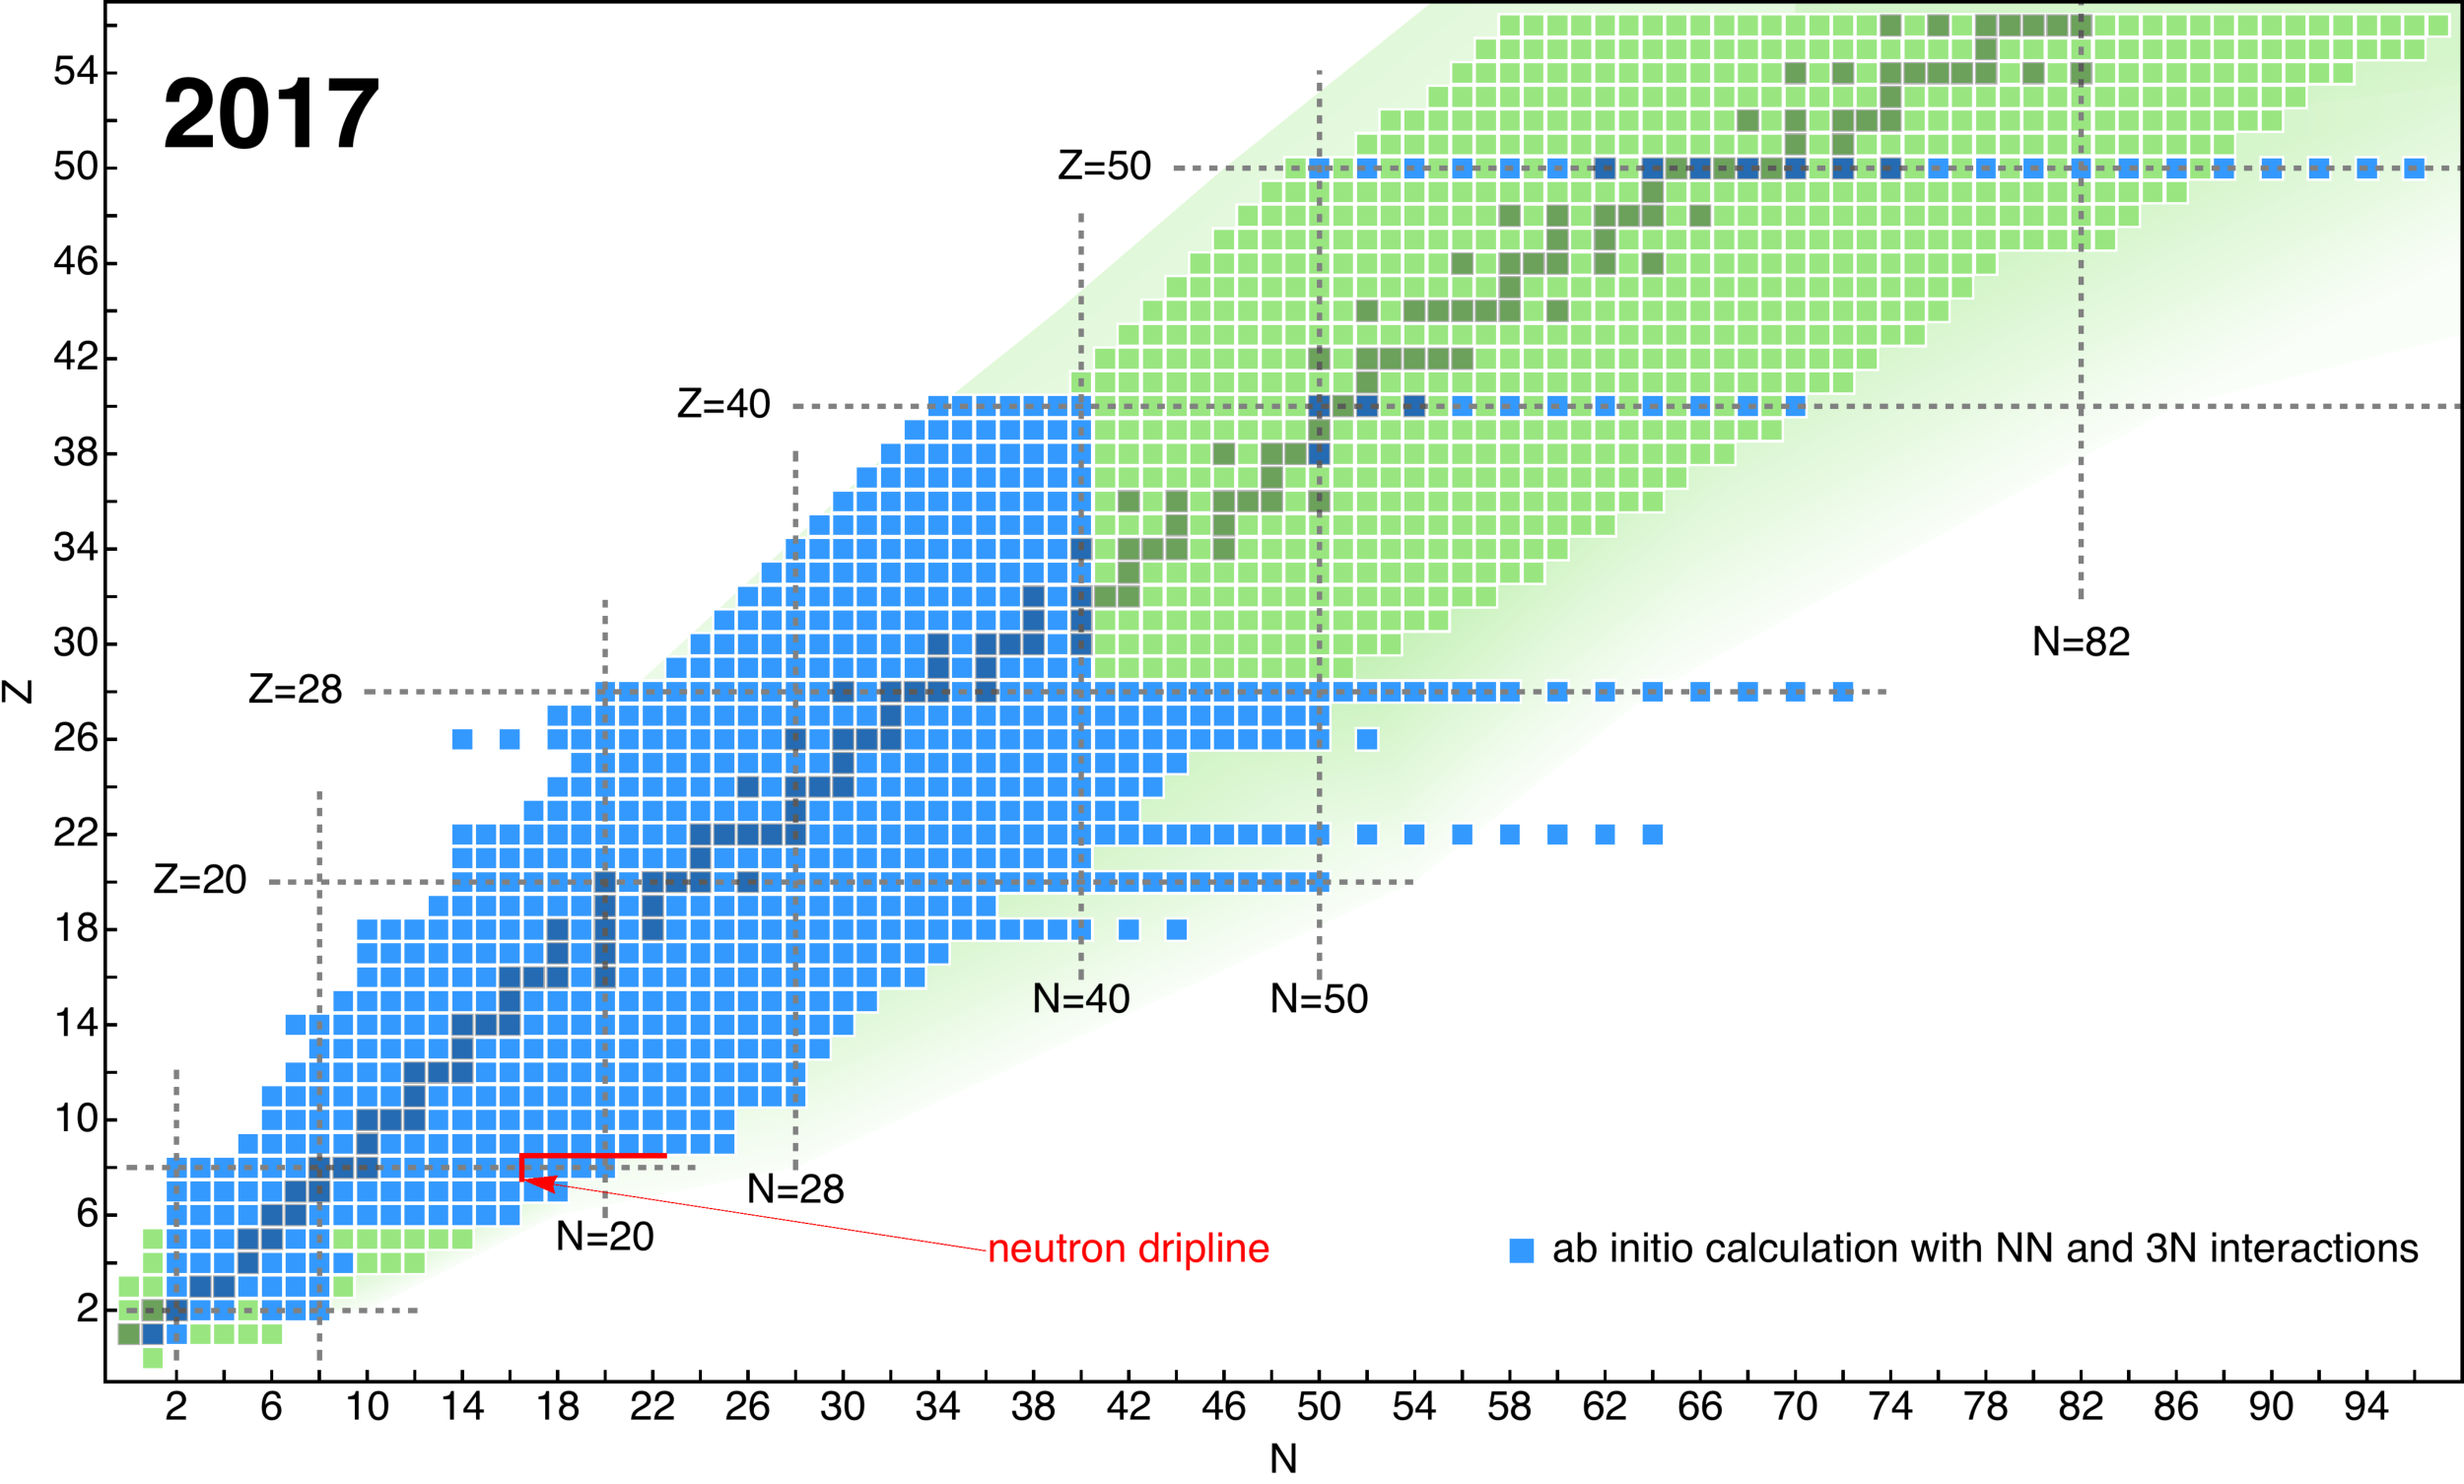
\includegraphics[width=0.8\textwidth]{nuclear_chart_2017}};
\end{tikzpicture}

\tiny Images courtesy of Heiko Hergert
\end{center}
\end{frame}


\begin{frame}
\frametitle{The Similarity Renormalization Group}
The similarity renormalization group (SRG) is an RG method which performs a continuous unitary transformation on an operator in order to:
\begin{itemize}
    \item Get rid of coupling between low and high energies
    \item Preserve low-energy observables (operator eigenvalues)
\end{itemize}
\pause

This transformation is given by:

\begin{equation}
\frac{d\hat{H}_s}{ds} = [\hat{\eta}_s, \hat{H}_s] = [[\hat{G}_s, \hat{H}_s], \hat{H}_s]
\end{equation}

where:\pause
\begin{itemize}
    \item $\hat{\eta}_s$ is the generator of the transformation\pause
    \item $\hat{G}_s$ is the flow operator, given by the user, which dictates the form to which the operator evolves\pause
    \item $s$ is the flow parameter, which goes from $s=0$ towards $s=\infty$ over the course of an SRG evolution
\end{itemize}
\end{frame}

\begin{frame}
\frametitle{Benefits of SRG}
A typical example of an application of the SRG to a calculation looks like:
\begin{enumerate}
    \item Start with 2-body or 3-body operator in a large basis
    \item Apply SRG to drive operator towards the diagonal
    \item Truncate basis, keeping low-energy sector and discarding high-energy sector
    \item Embed 2-body or 3-body operator in $A$-body
    \item Compute desired $A$-body observable
\end{enumerate}
\pause
\begin{alertblock}{Problem Size Reduction}
Truncating the basis in the 2-body or 3-body space greatly reduces the size of the resulting $A$-body space, thus making calculations of $A$-body observables feasible.
\end{alertblock}
\end{frame}


\begin{frame}
\frametitle{Limits of SRG}
While the SRG evolution of an $A$-body operator is unitary when done in the $A$-body space, it induces many-body forces that are seen when embedding the $A$-body operator in the basis for a larger system. These many-body forces:
\begin{itemize}
    \item Change the eigenvalues of the operator
    \item Are in general not possible to fully account for
    \item Show up as an error in the computed observables
    \item Scale with the size of the full system, limiting the application of SRG to small and medium systems
\end{itemize}
\pause
\begin{alertblock}{Alternative Flow Operators}
Currently, the kinetic energy, $\hat{T}$, is used as the flow operator, $\hat{G}_s$, for nearly all SRG calculations. Alternative choices for $\hat{G}_s$ many induce fewer many-body forces, extending the range of SRG to heavier isotopes.
\end{alertblock}
\end{frame}

\begin{frame}
\frametitle{1-Dimensional Setting}
SRG was originally explored in the context of low-energy nuclear physics in a 1-dimensional system:
\begin{itemize}
    \item System of $A$ bosons
    \item Factor out center-of-mass behavior and focus on behavior relative to center-of-mass
    \item 2-body local potential, $V(p, p')$, given in terms of relative Jacobi momenta
    \item Transform to discrete harmonic oscillator basis to embed 2-body potential in $A$-body system
\end{itemize}
\end{frame}

\begin{frame}
\frametitle{Harmonic Oscillator Basis}
Harmonic oscillator (HO) states are the eigenstates to the ``particle in a 1-dimensional harmonic oscillator potential" problem:
\begin{equation}
\hat{H}_{HO}\ket{n} = E_n\ket{n}
\end{equation}
\pause
For a system of $A$ particles, the general state is a product state of single-particle eigenstates:
\begin{equation}
\ket{n_1,n_2,...n_A} = \prod_{i=1}^A\ket{n_i}
\end{equation}
\pause
When working with relative Jacobi coordinates:
\begin{itemize}
    \item Define harmonic oscillator states to be with respect to Jacobi momenta
    \item Require $A-1$ Jacobi coordinates and thus product states of $A-1$ HO states
\end{itemize}
\end{frame}

\begin{frame}
\frametitle{Symmetrizing the HO Basis}
\begin{alertblock}{Spin-statistics theorem}
The state of any system of identical bosons must be symmetric under any permutation of the particles.
\end{alertblock}

\pause

We can create an $A$-body basis of HO product states that reflect this condition by:
\begin{itemize}
    \item Diagonalizing the 2-body symmetrizer, $S = (1 + P_{12})/2$, and selecting the eigenstates with eigenvalue 1 to get our 2-body basis
    \item Generating a set of $A$-body product states from the symmetrized $(A-1)$-body basis
    \item Getting the $A$-body states by diagonalizing the $A$-body symmetrizer
\end{itemize}\pause
In this work, we do this to get symmetrized 2-body and 3-body bases.
\end{frame}

\begin{frame}
\frametitle{The Negele Potential}
\begin{alertblock}{Negele Potential}
\begin{equation}
\hat{V}(p, p') = \frac{V_1}{2\pi\sqrt2}e^{-(p-p')^2\sigma_1^2/8} + \frac{V_2}{2\pi\sqrt2}e^{-(p-p')^2\sigma_2^2/8}
\end{equation}
\end{alertblock}
We use two parametrizations of the Negele potential:
\begin{itemize}
    \item $\hat{V}_\alpha$ is nuclear-like, with a mid-range attractive part and a short-range repulsive part
    \item $\hat{V}_\beta$ is purely attractive
\end{itemize}
\end{frame}

\begin{frame}
\frametitle{2-Body Momentum Space SRG}
With both $\hat{T}$ as the flow operator and an alternative block diagonal flow operator, we see SRG achieve the desired decoupling of low and high momenta:


\vspace{\baselineskip}
With $\hat{G}_s = \hat{T}$:
\begin{center}
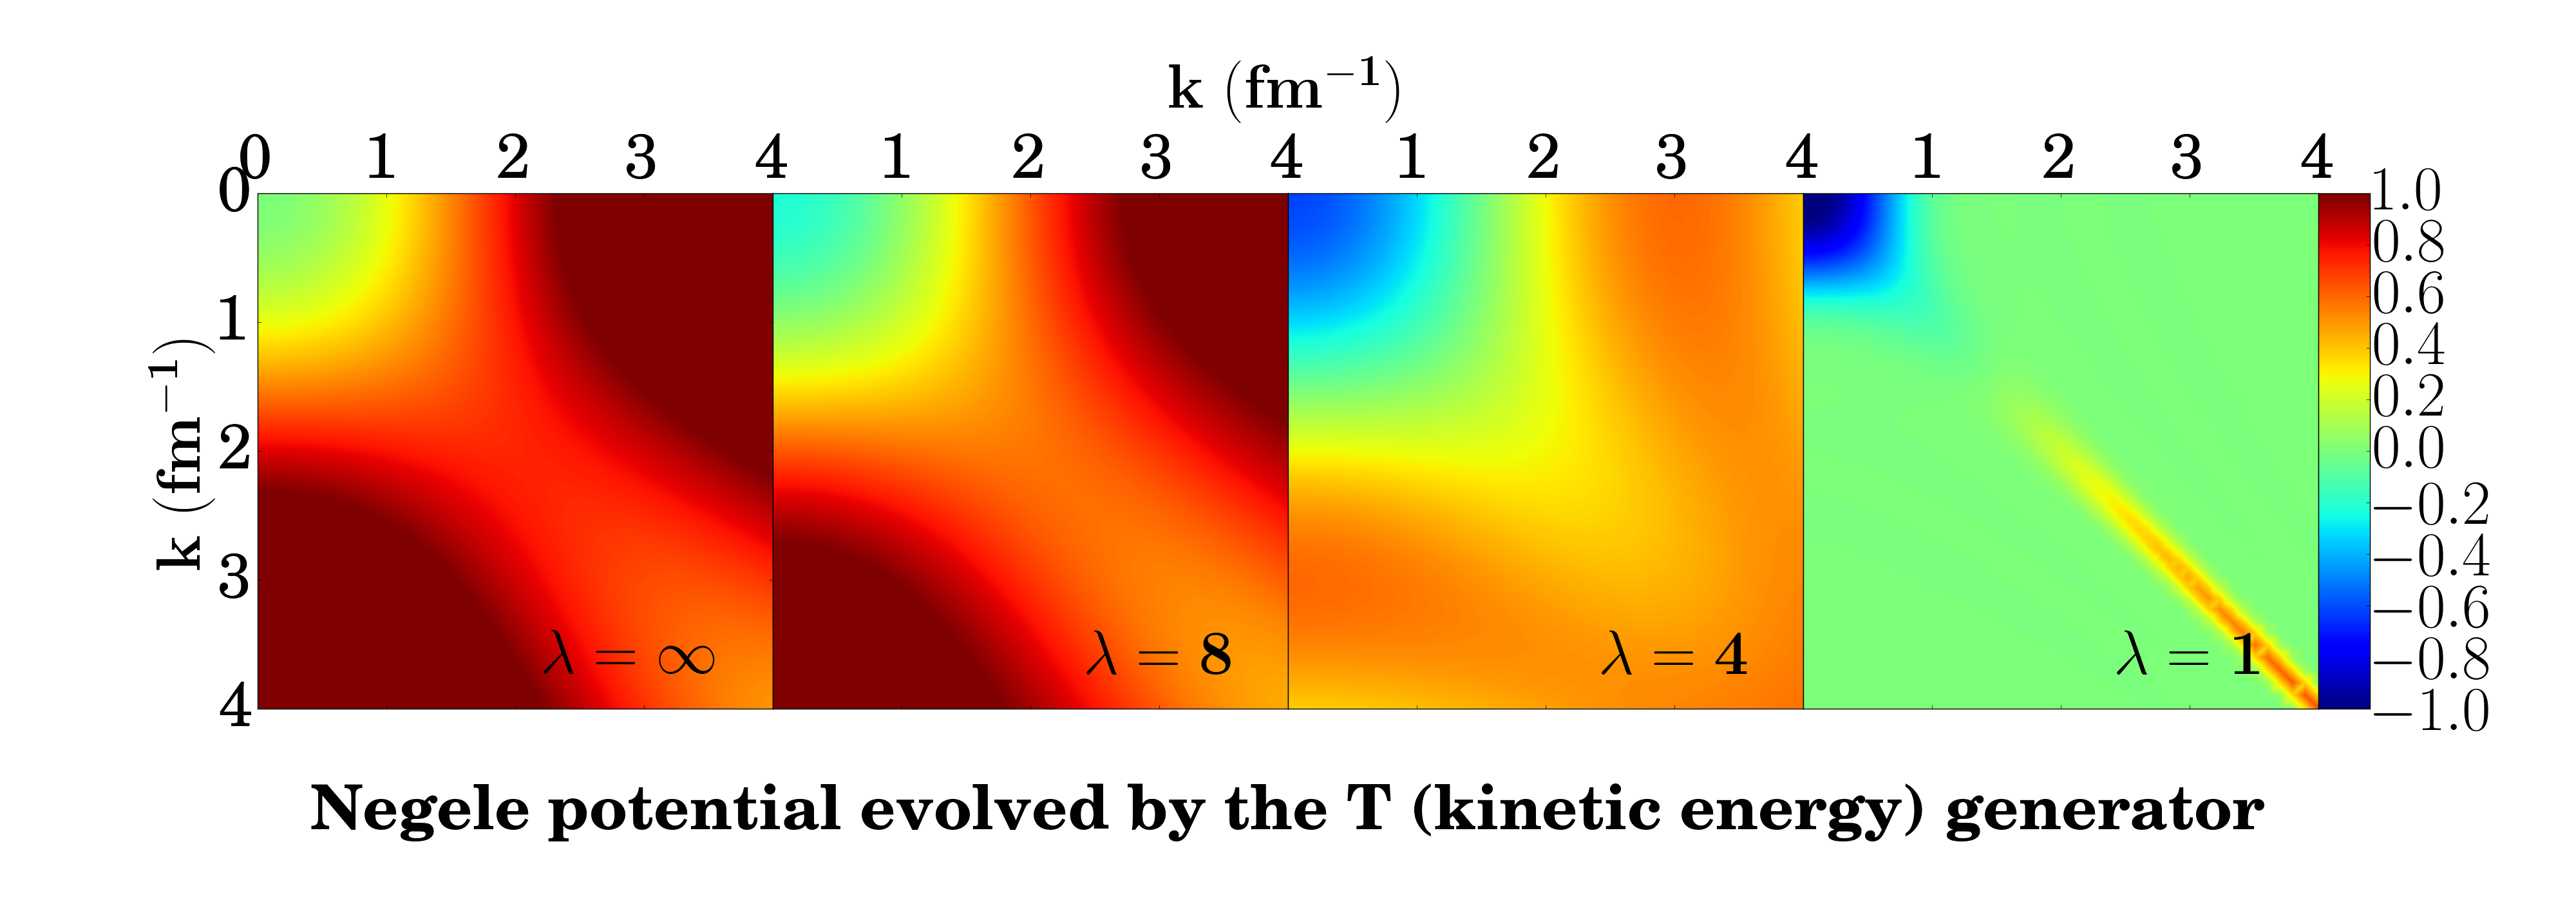
\includegraphics[trim={0 5cm 0 0},clip,width=0.95\textwidth]{T_evolution}
\end{center}

\end{frame}

\begin{frame}
\frametitle{2-Body Momentum Space SRG}
With both $\hat{T}$ as the flow operator and an alternative block diagonal flow operator, we see SRG achieve the desired decoupling of low and high momenta:

\vspace{\baselineskip}
With $\hat{G}_s = \hat{H}_{BD}$:
\begin{center}
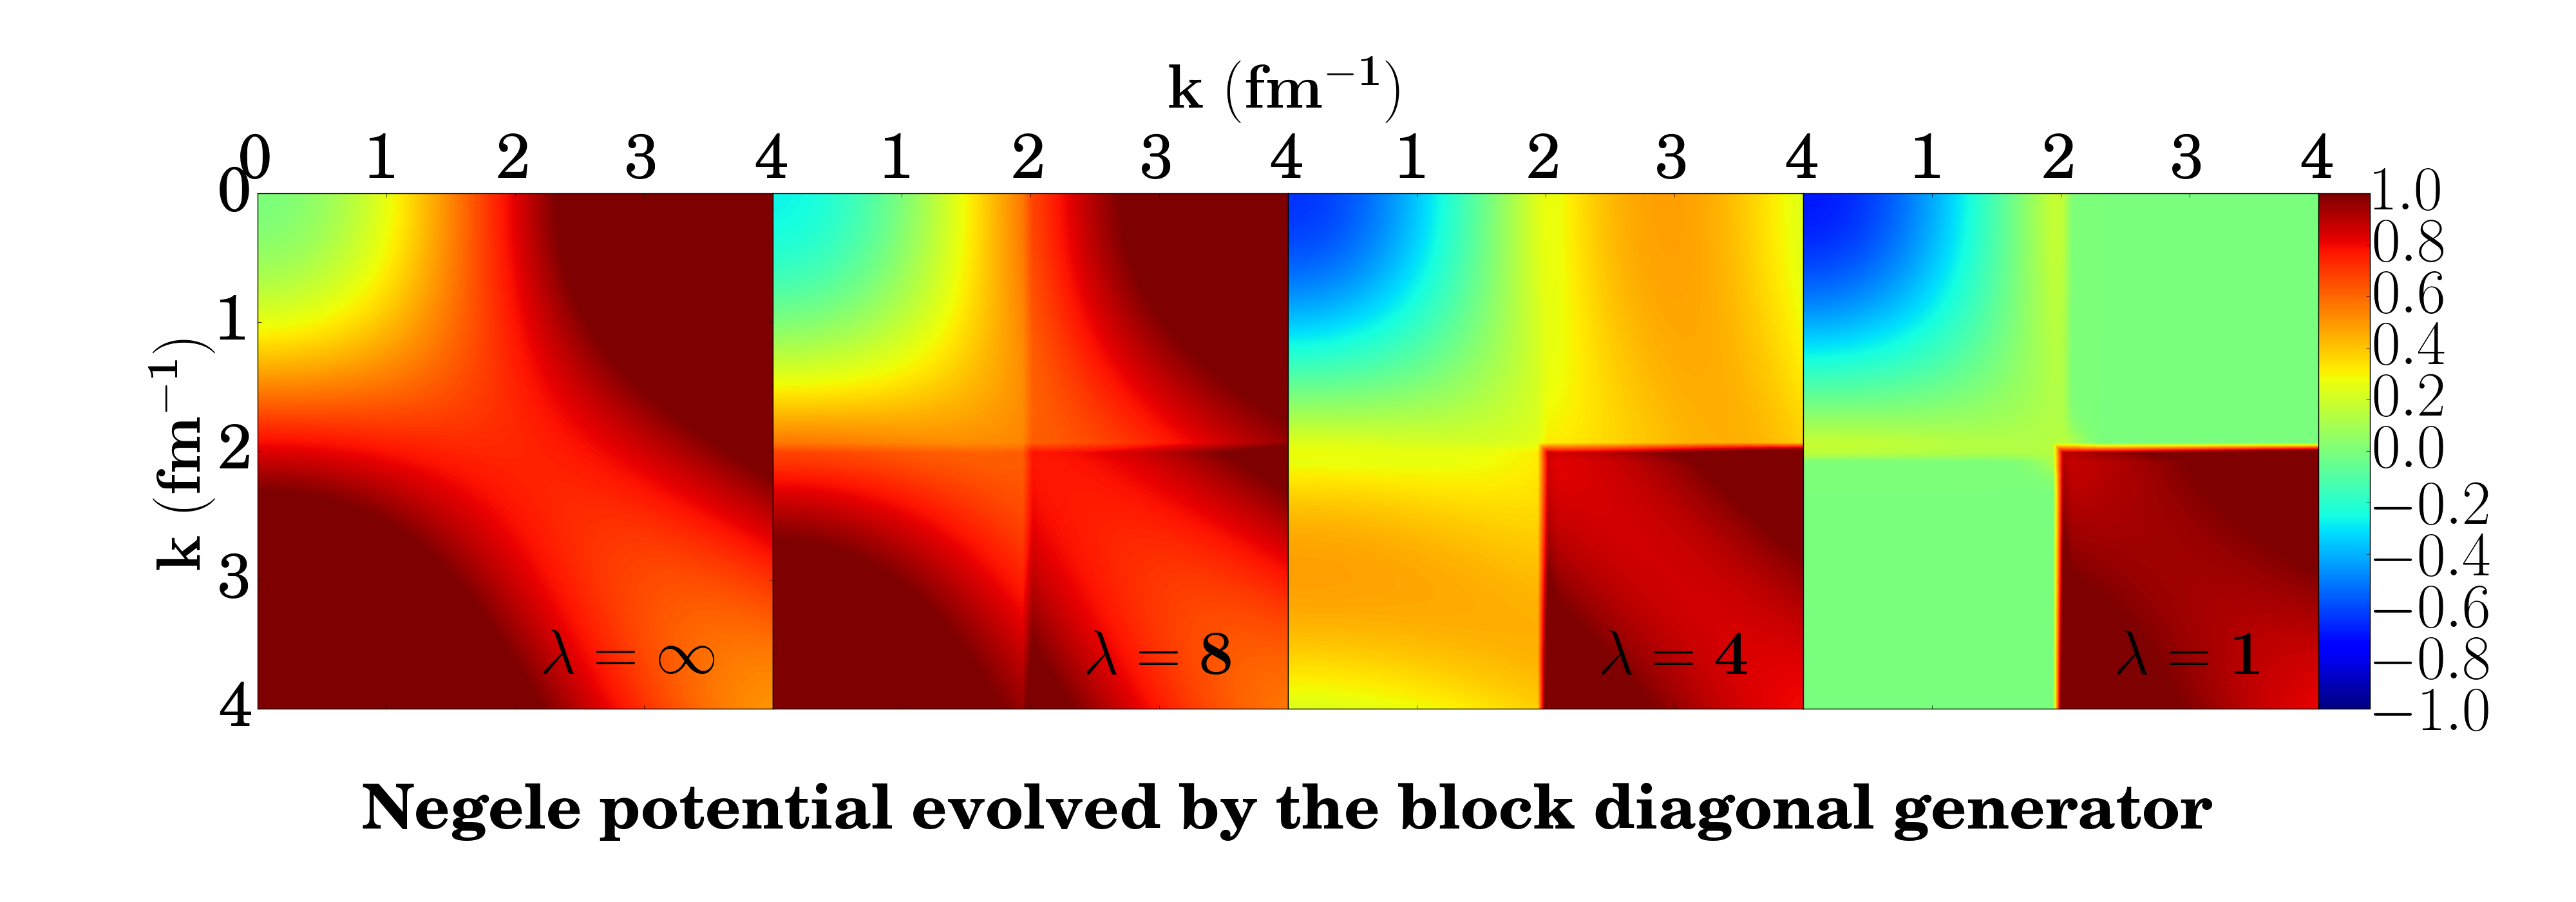
\includegraphics[trim={0 5cm 0 0},clip,width=0.95\textwidth]{BD_1_evolution}
\end{center}

\end{frame}

\begin{frame}
\frametitle{Transformation to HO Space}
When transforming operators to HO space, we must pick a value of $N_{max}$ such that our low-energy observables are converged to their true values. These figures focus on $\hat{V}_\alpha$ since $\hat{V}_\beta$ converges much faster. We find $N_{max}=28$ to be sufficient for the 2-body and 3-body ground state energies.

\begin{figure}
\begin{center}
\subfloat[2-body]{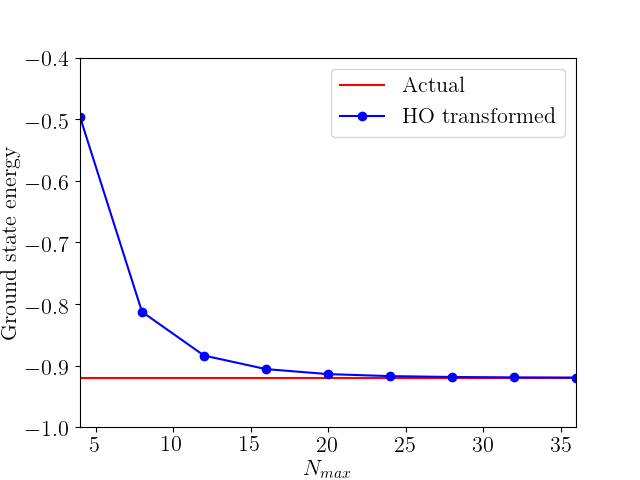
\includegraphics[width=0.5\linewidth]{alpha_2body_nmax}}
\subfloat[3-body]{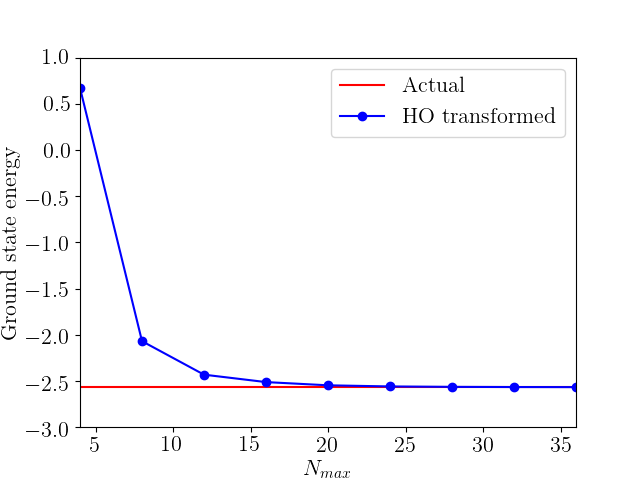
\includegraphics[width=0.5\linewidth]{alpha_3body_nmax}}
\end{center}
\end{figure}

\end{frame}

\begin{frame}
\frametitle{Induced 3-Body Force with $G_s=T$}
We find a large 3-body force induced by the 2-body SRG evolution with $\hat{G}_s=\hat{T}$.

\begin{figure}
\begin{center}
\subfloat[$\hat{V}_\alpha$\label{fig:heinz_va}]{\centering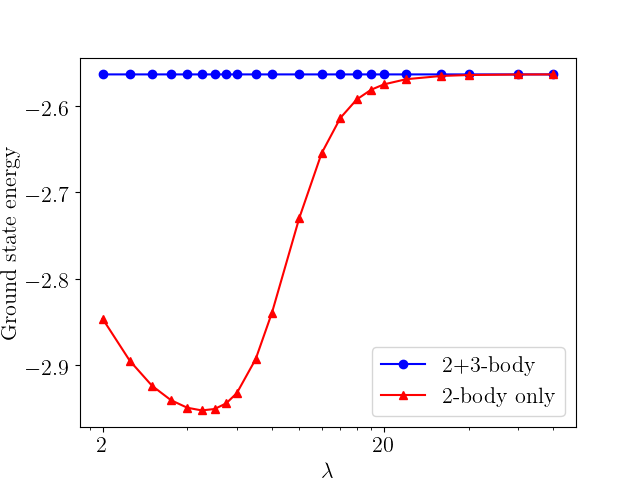
\includegraphics[width=0.5\linewidth]{manybody_T_alpha}}
\subfloat[$\hat{V}_\beta$\label{fig:heinz_vb}]{\centering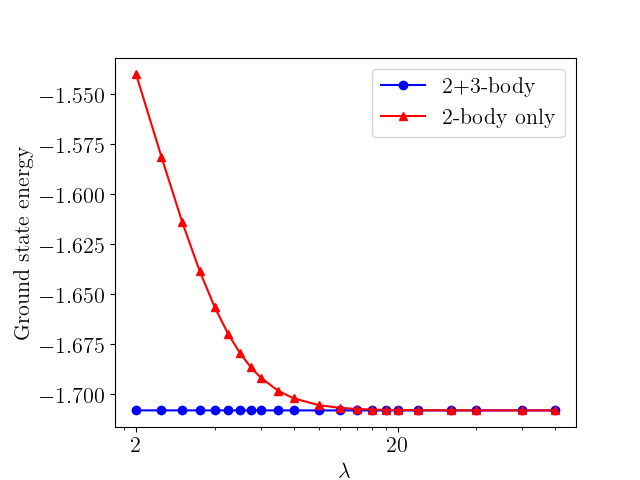
\includegraphics[width=0.5\linewidth]{manybody_T_beta}}
\end{center}
\label{fig:heinz_vfull}
\end{figure}
\end{frame}

\begin{frame}
\frametitle{Induced 3-Body Force with Alternative Flow Operator}
We define an alternative flow operator, $\hat{H}_{BDHO}$, that is block-diagonal in HO space:
\begin{equation}
\hat{G}_s = \hat{H}_{BDHO} = \hat{T} + \hat{V} \Theta(N - \Lambda) \Theta(N' - \Lambda),
\end{equation}
where $\Lambda$ is the harmonic oscillator cutoff for the low-energy sector.

\pause
\begin{figure}
\begin{center}
\subfloat[$\hat{V}_\alpha$\label{fig:heinz_newa}]{\centering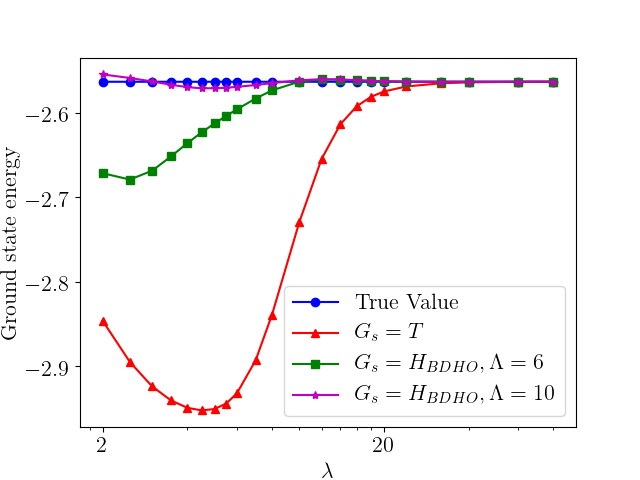
\includegraphics[width=0.5\linewidth]{new_alpha}}
\subfloat[$\hat{V}_\beta$\label{fig:heinz_newb}]{\centering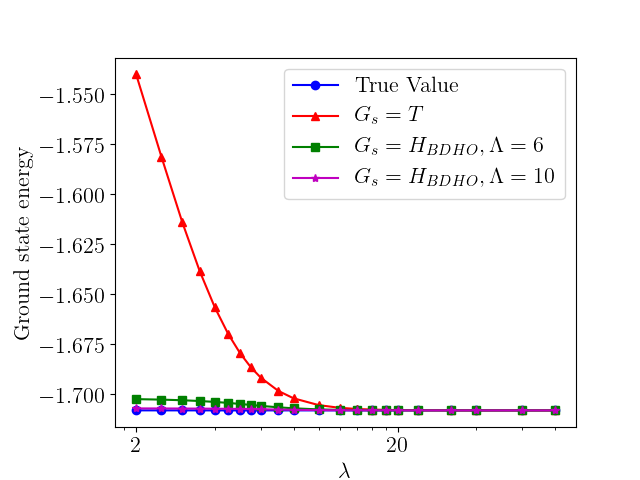
\includegraphics[width=0.5\linewidth]{new_beta}}
\end{center}
\label{fig:heinz_newfull}
\end{figure}

\end{frame}

\begin{frame}
\frametitle{\texttt{srg1d}}
\texttt{srg1d} is the Python framework behind this work.
\begin{itemize}
    \item Validated against previous results for 2-body and 3-body cases
    \item Abstracts technical details (basis construction and symmetrization, operator embedding, etc.) from user
    \item Simplifies writing SRG calculations
    \item Testing a new flow operator requires user to change 2 lines of code in an existing script
\end{itemize}
\vspace{\baselineskip}
With \texttt{srg1d}, further exploration of this 1-dimensional setting is made easy.
\end{frame}

\begin{frame}
\frametitle{Conclusions and Future Work}
Conclusions:
\begin{itemize}
    \item Validated implementation against previous results
    \item Alternative flow operator results are preliminary
    \begin{itemize}
        \item Need to compare rate of decoupling between different flow operators
        \item Need to explore 4-body and 5-body forces induced to see general trends
    \end{itemize}
    \item \texttt{srg1d} framework makes additional testing easy
\end{itemize}
\pause
Future Work:
\begin{itemize}
    \item Test proposed alternative flow operators further
    \item Formulate new flow operators with different features
    \item Seek to understand what features of flow operators are desirable
\end{itemize}

\end{frame}

\appendix

\backupbegin
% backup slides
\begin{frame}
\frametitle{2-Body $V_\alpha$ vs. $V_\beta$}
\begin{figure}
\begin{center}
\subfloat[$\hat{V}_\alpha$]{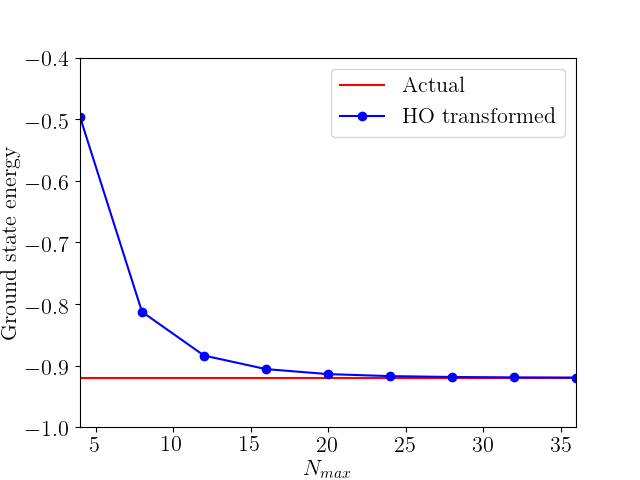
\includegraphics[width=0.5\linewidth]{alpha_2body_nmax}}
\subfloat[$\hat{V}_\beta$]{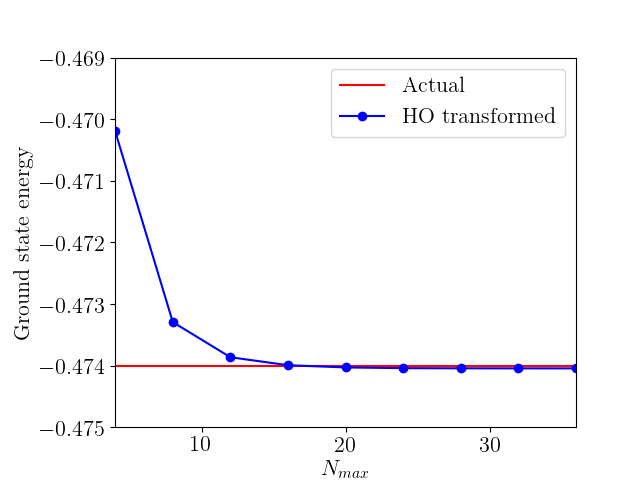
\includegraphics[width=0.5\linewidth]{beta_2body_nmax}}
\end{center}
\end{figure}
\end{frame}

\begin{frame}
\frametitle{3-Body $V_\alpha$ vs. $V_\beta$}
\begin{figure}
\begin{center}
\subfloat[$\hat{V}_\alpha$]{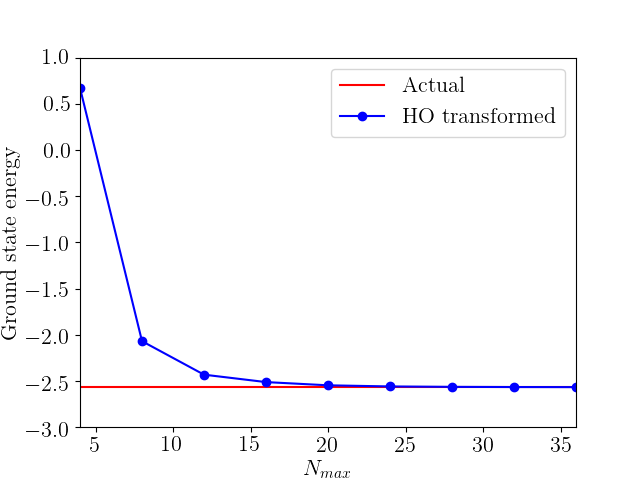
\includegraphics[width=0.5\linewidth]{alpha_3body_nmax}}
\subfloat[$\hat{V}_\beta$]{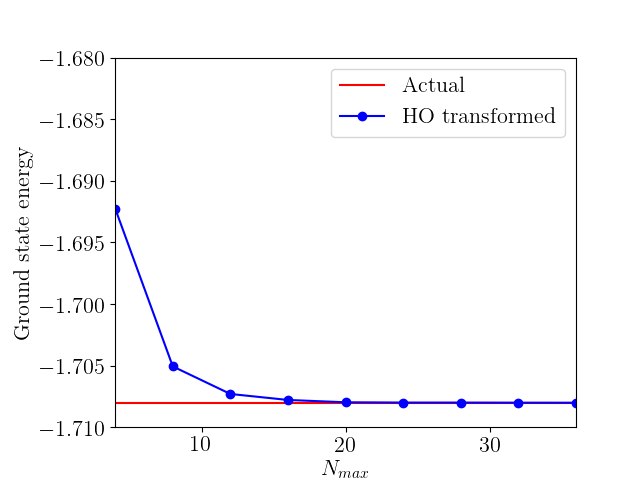
\includegraphics[width=0.5\linewidth]{beta_3body_nmax}}
\end{center}
\end{figure}
\end{frame}

\begin{frame}
\frametitle{$\omega$ Optimization}
\begin{figure}
\begin{center}
\subfloat[2-body ground state energy\label{fig:2body_a_w}]{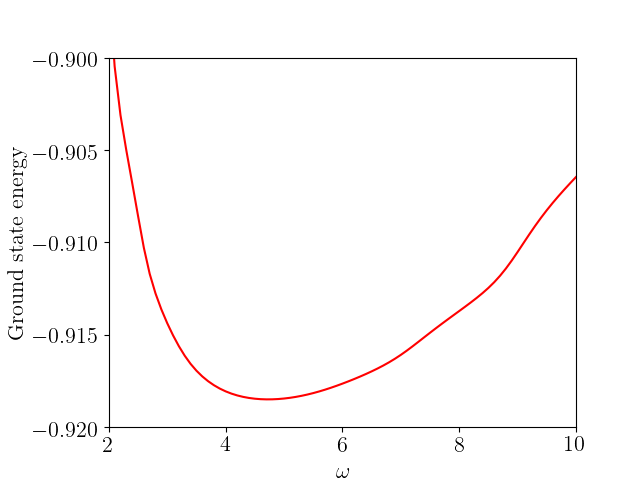
\includegraphics[width=0.5\linewidth]{alpha_2body_w}}
\subfloat[3-body ground state energy\label{fig:3body_a_w}]{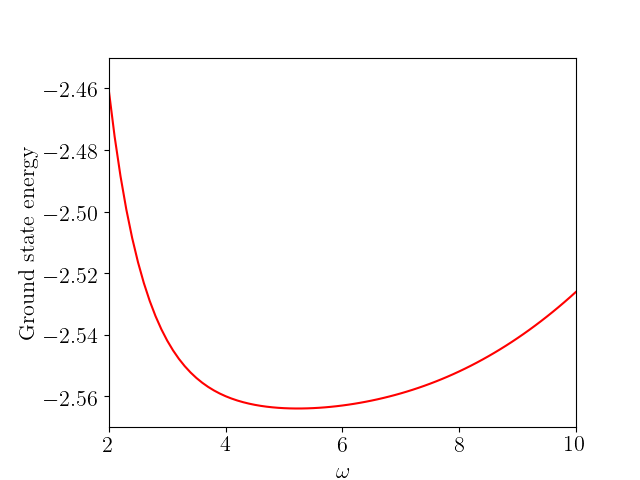
\includegraphics[width=0.5\linewidth]{alpha_3body_w}}
\end{center}
\label{fig:alpha_w}
\end{figure}
\end{frame}


\backupend

\end{document}
